\section{Auswertung}
\label{sec:Auswertung}
\subsection{Bestimmung der zeitkonstante bei konstanter Frequenz}
Die Bestimmung der Zeitkonstante $RC$ erfolgt mit der
Auswertung einer Entladungskurve. Dazu werden die Messdaten aus
\autoref{tab:Messdaten1} in einem halblogarhithmierten Diagramm in
\autoref{fig:fit1} dargestellt. Außerdem wird eine linearer Fit 
mittels Scipy berechnet und durch die Messdaten gelegt.
 \begin{table}[H]
    \centering
    \label{tab:Messdaten1}
    \caption{Messdaten der Entladekurve eines Kondensators im RC-Kreis.}
    \begin{tblr}{colspec={c c||c c}}
        \toprule
        $t$\,\,/\,\,s & $U$\,\,/\,\,V &  $t$\,\,/\,\,s & $U$\,\,/\,\,V\\
        \midrule
        -1.3 &  3.8 & -0.5 & -1.4\\
        -1.2 &  3.0 & -0.4 & -1.7\\
        -1.1 &  1.9 & -0.3 & -1.9\\
        -1.0 &  1.1 & -0.2 & -2.1\\
        -0.9 &  0.5 & -0.1 & -2.6\\
        -0.8 &  0.0 &  0.0 & -2.8\\
        -0.7 & -0.2 &  0.1 & -3.2\\
        -0.6 & -0.9 &  0.2 & -3.5\\
        \bottomrule
    \end{tblr}
\end{table}
\begin{figure}[H]
    \centering
    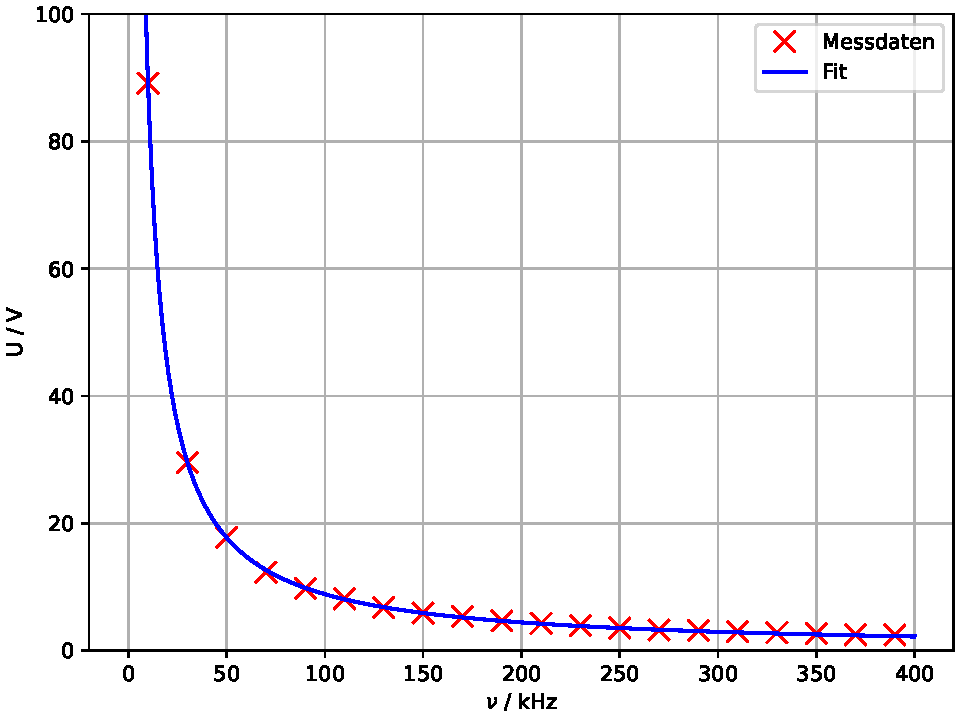
\includegraphics[width=\textwidth]{build/plota.pdf}
    \label{fig:fit1}
    \caption{Der Logarhithmus der Spannung geteilt durch die Ausgangsspannung $U_0=\qty{3.5}{\volt}$ 
    aufgetragen gegen die Zeit.}
\end{figure}\noindent
Für den Fit werden zu den Messdaten der Zeit jeweils $\qty{1.3}{\milli\second}$ dazu addiert
sowie zu den Spannungen jeweils $\qty{3.5}{\volt}$, sodass die Kurve bei $t=0$ beginnt und bei 
$U=0$ endet. Am Verlauf und der Steigung ändert dies nichts. Ebenso wurde der letzte Messwert, 
in der Tabelle zu finden bei $\qty{0.2}{\milli\second}$, aus der Berechnung herausgelassen. Weiteres 
dazu in der Diskussion. 
Die Koeffizienten der linearen Funktion $f(x)=ax+b$ werden berechnet als
\begin{align*}
    a&=\qty{-1.9(0.14)}{\per\milli\second}\\
    \intertext{und}
    b&=0.2\pm0.1\,.
\end{align*}
Die Steigung der Geraden ist hier $\sfrac{1}{RC}$, also gilt
\begin{align*}
    \frac{1}{RC}&=a\Leftrightarrow RC=\frac{1}{a}\\
    \Rightarrow RC&=\qty{0.52(0.04)}{\milli\second}\,.
\end{align*}
Die Unsicherheiten aller Größen wird mittels Python und der Gaußschen 
Fehlerfortpflanzung berechnet. Die Formel dafür lautet
\begin{equation}
    \increment f= \sqrt{\sum_{i=1}^n\left(\frac{\partial f}{\partial x_i}
    \right)^2\cdot (\increment x_i)^2}\,.
    \end{equation}
Dabei ist $f$ die zur Berechnung genutzte Formel, $x_i$ dessen
Variablen und $\increment x_i$ die jeweilige Unsicherheit.
Dr letzte Messwert der messreihe wurde nicht in die Berechnung von $RC$ miteinbezogen,
näheres dazu in der Diskussion.
\subsection{Bestimmung der Zeitkonstante bei variierter Frequenz}
Wie in der Durchführung bereits beschrieben, wird in dieser Messreihe unter anderem die 
Frequenzabhängigkeit einer Ausgangsamplitude gemessen. Die dazu gemessenen Werte sind in 
\autoref{tab:Messdaten2} aufgeführt.
\begin{table}
    \centering
    \label{tab:Messdaten2}
    \caption{Erreger- und Ausgangsspannung in Abhängigkeit der Frequenz.} 
    \begin{tblr}{colspec={c c c||c c c}}
        \toprule
        $f$\,\,/\,\,$\unit{\hertz}$ & $U_\text{E}$\,\,/\,\,V & $U_\text{A}$\,\,/\,\,V&
        $f$\,\,/\,\,$\unit{\hertz}$ & $U_\text{E}$\,\,/\,\,V & $U_\text{A}$\,\,/\,\,V\\
        \midrule
        5.04 & 4.0 & 4.000 & 505  & 4.0 & 0.500\\
        55   & 4.0 & 3.000 & 1000 & 4.0 & 0.300\\
        105  & 4.0 & 2.200 & 1500 & 4.0 & 0.200\\
        155  & 4.0 & 1.800 & 2000 & 4.0 & 0.180\\
        205  & 4.0 & 1.200 & 2500 & 4.0 & 0.110\\
        305  & 4.0 & 1.000 & 3000 & 4.0 & 0.105\\
        355  & 4.0 & 0.800 & 4000 & 4.0 & 0.090\\
        405  & 4.0 & 0.700 & 5000 & 4.0 & 0.060\\
        455  & 4.0 & 0.600 &      &     &      \\
        \bottomrule
    \end{tblr}
\end{table}
Wie schon zu erwarten, bleibt die Eingangsspannung während der kompletten Messreihe konstant. 
Die Ausgangsspannung soll nach \autoref{eq:arctan} abfallen. Diese Gleichung wird noch wie folgt umgestellt
\begin{equation}
    \frac{A(\omega)}{U_0}=\frac{1}{\sqrt{1+\omega^2R^2C^2}}\,.
    \label{eq:fit2}
\end{equation}
Um das Frequenzverhalten zu überprüfen, werden die gemessenen Ausgangsspannungen also durch $U_0$ geteilt.
Anschließend wird nach Formel \ref{eq:fit2} eine Funktion durch die Messdaten gefittet um die Zeitkonstante 
zu bestimmen. Da der Versuchsaufbau unverändert ist, sollte sich auch die Zeitkonstante nicht verändert haben.
Dies wird mittels des in \autoref{fig:fit2} gezeigten Fits und der damit einhergehenden Berechnung von $RC$
geprüft beziehungsweise berechnet.
\begin{figure}[H]
    \centering
    \label{fig:fit2}
    \caption{Die Ausgangsspannung geteilt durch die Erregerspannung aufgetragen gegen die Frequenz
    sowie eine nichtlineare Regression.}
    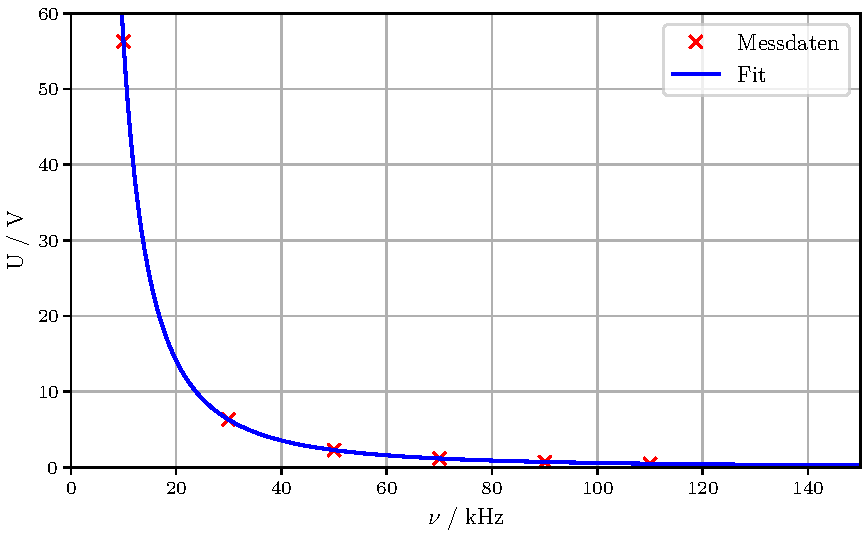
\includegraphics[width=\textwidth]{build/plotb.pdf}
\end{figure}\noindent
Für die Zeitkonstante ergibt sich mittels Scipy und integrierter Gaußscher Fehlerfortpflanzung für den 
Betrag der Zeitkonstante
\begin{equation}
    RC=\qty{2.27(0.05)}{\milli\second}\,.
\end{equation}
Hierbei ist $U_0=\qty{4}{\volt}$. 
\subsection{Phasenverschiebung des RC-Kreises}
Wie schon in der Theorie beschrieben, kommt es für hohe Frequenzen zu einer Phasenverschiebung
zwischen Ein- und Ausgangssignal. Zur Periodenlänge $b$ und der Phasenverschiebung $a$ in
Abhängigkeit der Frequenz wurden die in \autoref{tab:Phasenverschiebung} aufgeführten
Messwerte aufgenommen.
\begin{table}
    \centering
    \label{tab:Phasenverschiebung}
    \caption{Phasenverschiebung $a$ sowie Periodenlänge $b$ in Abhängigkeit dr Frequenz.}
    \begin{tblr}{colspec={c c c c ||c c c c}}
        \toprule
        $f$\,\,/\,\,Hz & $a$\,\,/\,\,ms & $b$\,\,/\,\,ms&$\varphi$\,\,/\,\,rad &
        $f$\,\,/\,\,Hz & $a$\,\,/\,\,ms & $b$\,\,/\,\,ms&$\varphi$\,\,/\,\,rad\\
        \midrule
        5.04 & 4.00&  156  & 0.16 & 505  & 0.20 & 0.60 & 1.05\\
        55   & 1.50 & 18.0 & 0.52 & 1000 & 0.20 & 0.40 & 1.57\\
        105  & 1.20 & 4.00 & 0.94 & 1500 & 0.10 & 0.15 & 2.09\\
        155  & 1.20 & 3.20 & 1.18 & 2000 & 0.08 & 0.20 & 1.26\\
        205  & 0.80 & 2.00 & 1.26 & 2500 & 0.06 & 0.15 & 1.26\\
        305  & 0.40 & 1.20 & 1.05 & 3000 & 0.05 & 0.12 & 1.31\\
        355  & 0.40 & 1.00 & 1.26 & 4000 & 0.04 & 0.10 & 1.26\\
        405  & 0.40 & 0.80 & 1.57 & 5000 & 0.04 & 0.08 & 1.57\\
        455  & 0.30 & 0.70 & 1.35 &      &      &      &     \\ 
        \bottomrule
    \end{tblr}
\end{table}
Die Perdiodenlänge $b$ wird hierbei über die Formel $b=\sfrac{1}{f}$ berechnet. Mit den gemessenen Daten soll 
eigentlich erneut die Zeitkonstante, jedoch diesmal über \autoref{eq:arctan1} bestimmt werden. Dies war mit 
den aufgeführten Messdaten jedoch leider nicht möglich. Näheres dazu ist in der Diskussion zu finden. 
Anstattdessen ist in \autoref{fig:plotc} der $\arctan(-\omega\cdot RC)$ mit dem Wert aus Teil b) für die 
Zeitkonstante geplottet.
\begin{figure}[H]
    \centering
    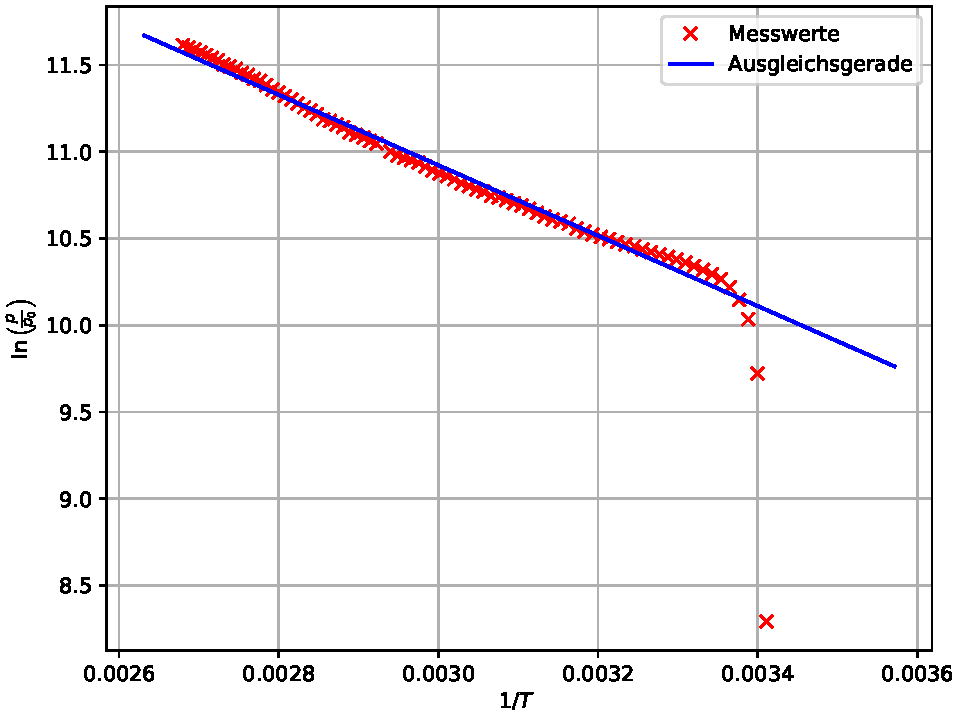
\includegraphics[width=\textwidth]{build/plotc.pdf}
    \caption{Gemessene Werte für die Phasenverschiebung $\varphi$ sowie die Theorie-Kurve.}
    \label{fig:plotc}
\end{figure}
\subsection{RC-Kreis als Integrator}
Wie in der Theorie schon diskutiert, lässt sich der RC-Kreis nach \autoref{eq:integrator} auch als Integrator verwenden. 
Um dies zu überprüfen, wurden drei verschiedene Schwingungsformen sowie deren Stammfunktionen auf das Oszilloskop gelegt.
Abb. \ref{fig:integration} zeigt diese.
\begin{figure}
    \begin{subfigure}{0.32\textwidth}
        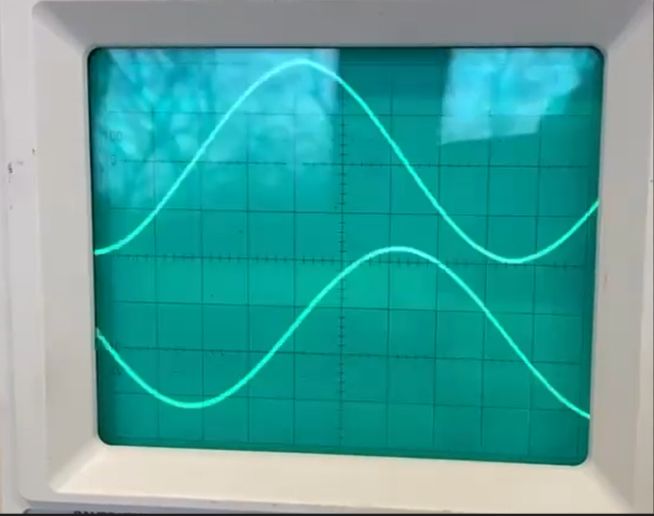
\includegraphics[height=3.5cm]{messdaten/cos_int.png}
        \caption{Sinusschwingung.}
    \end{subfigure}
    \hfill
    \begin{subfigure}{0.32\textwidth}
        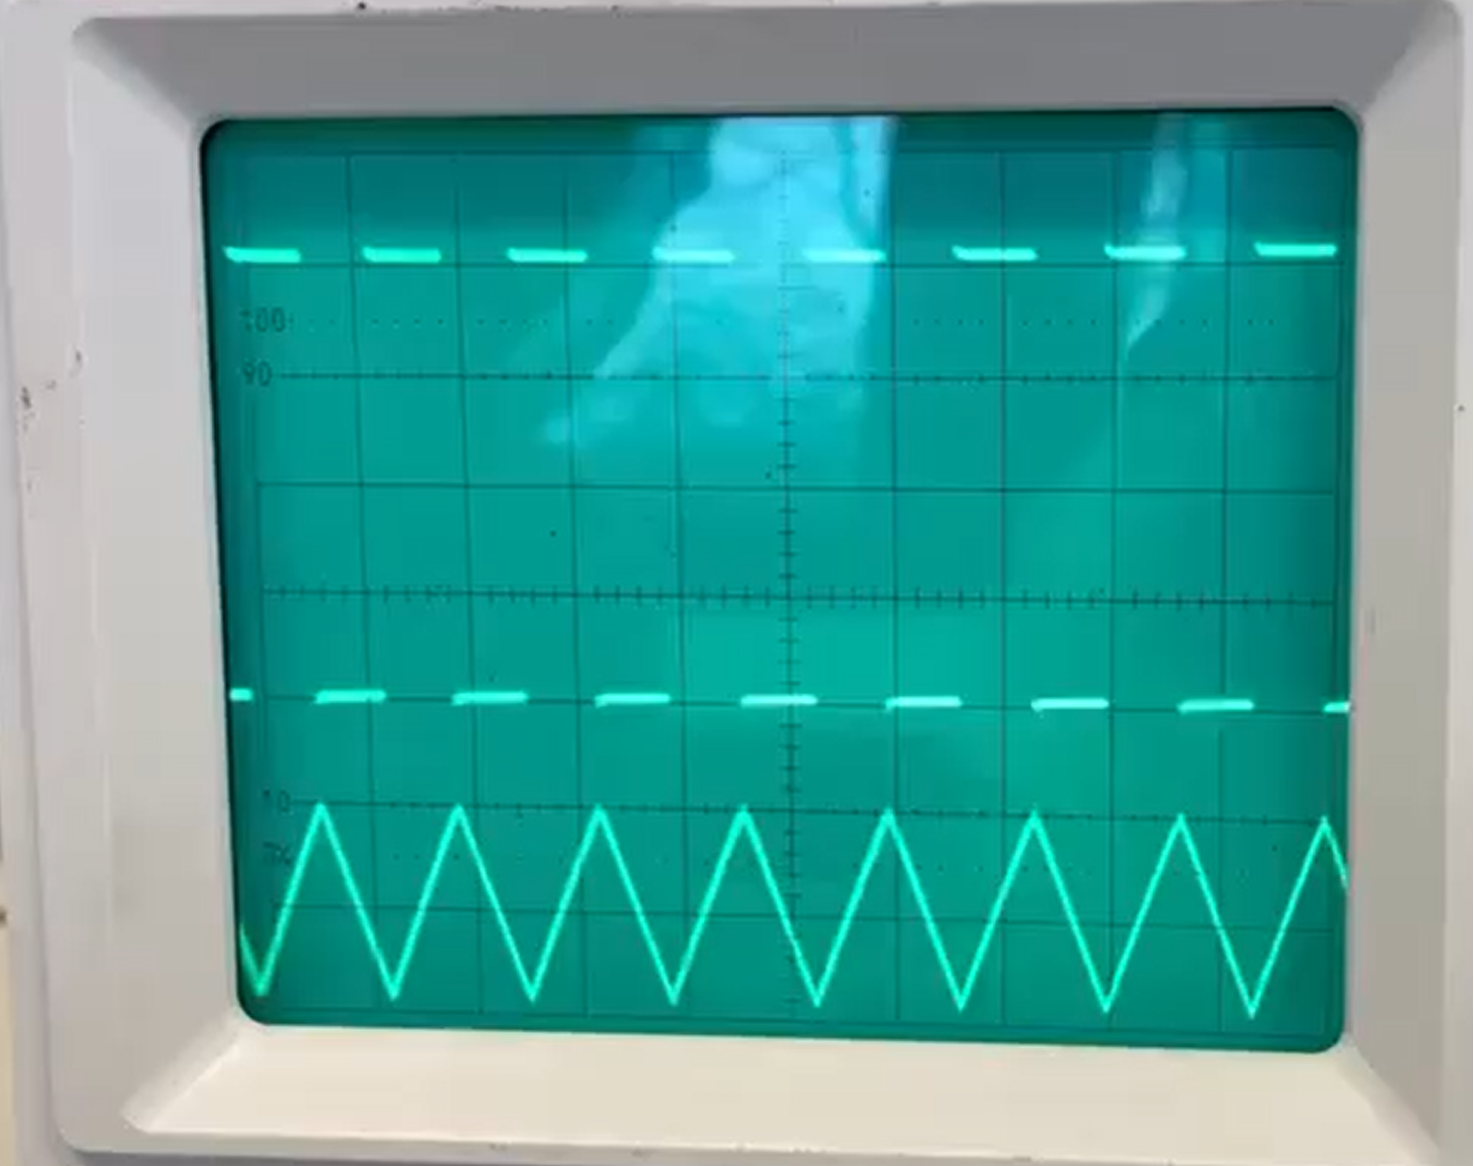
\includegraphics[height=3.5cm]{messdaten/dre_int.png}
        \caption{Rechtecksschwingung.}
    \end{subfigure}
    \hfill
    \begin{subfigure}{0.32\textwidth}
        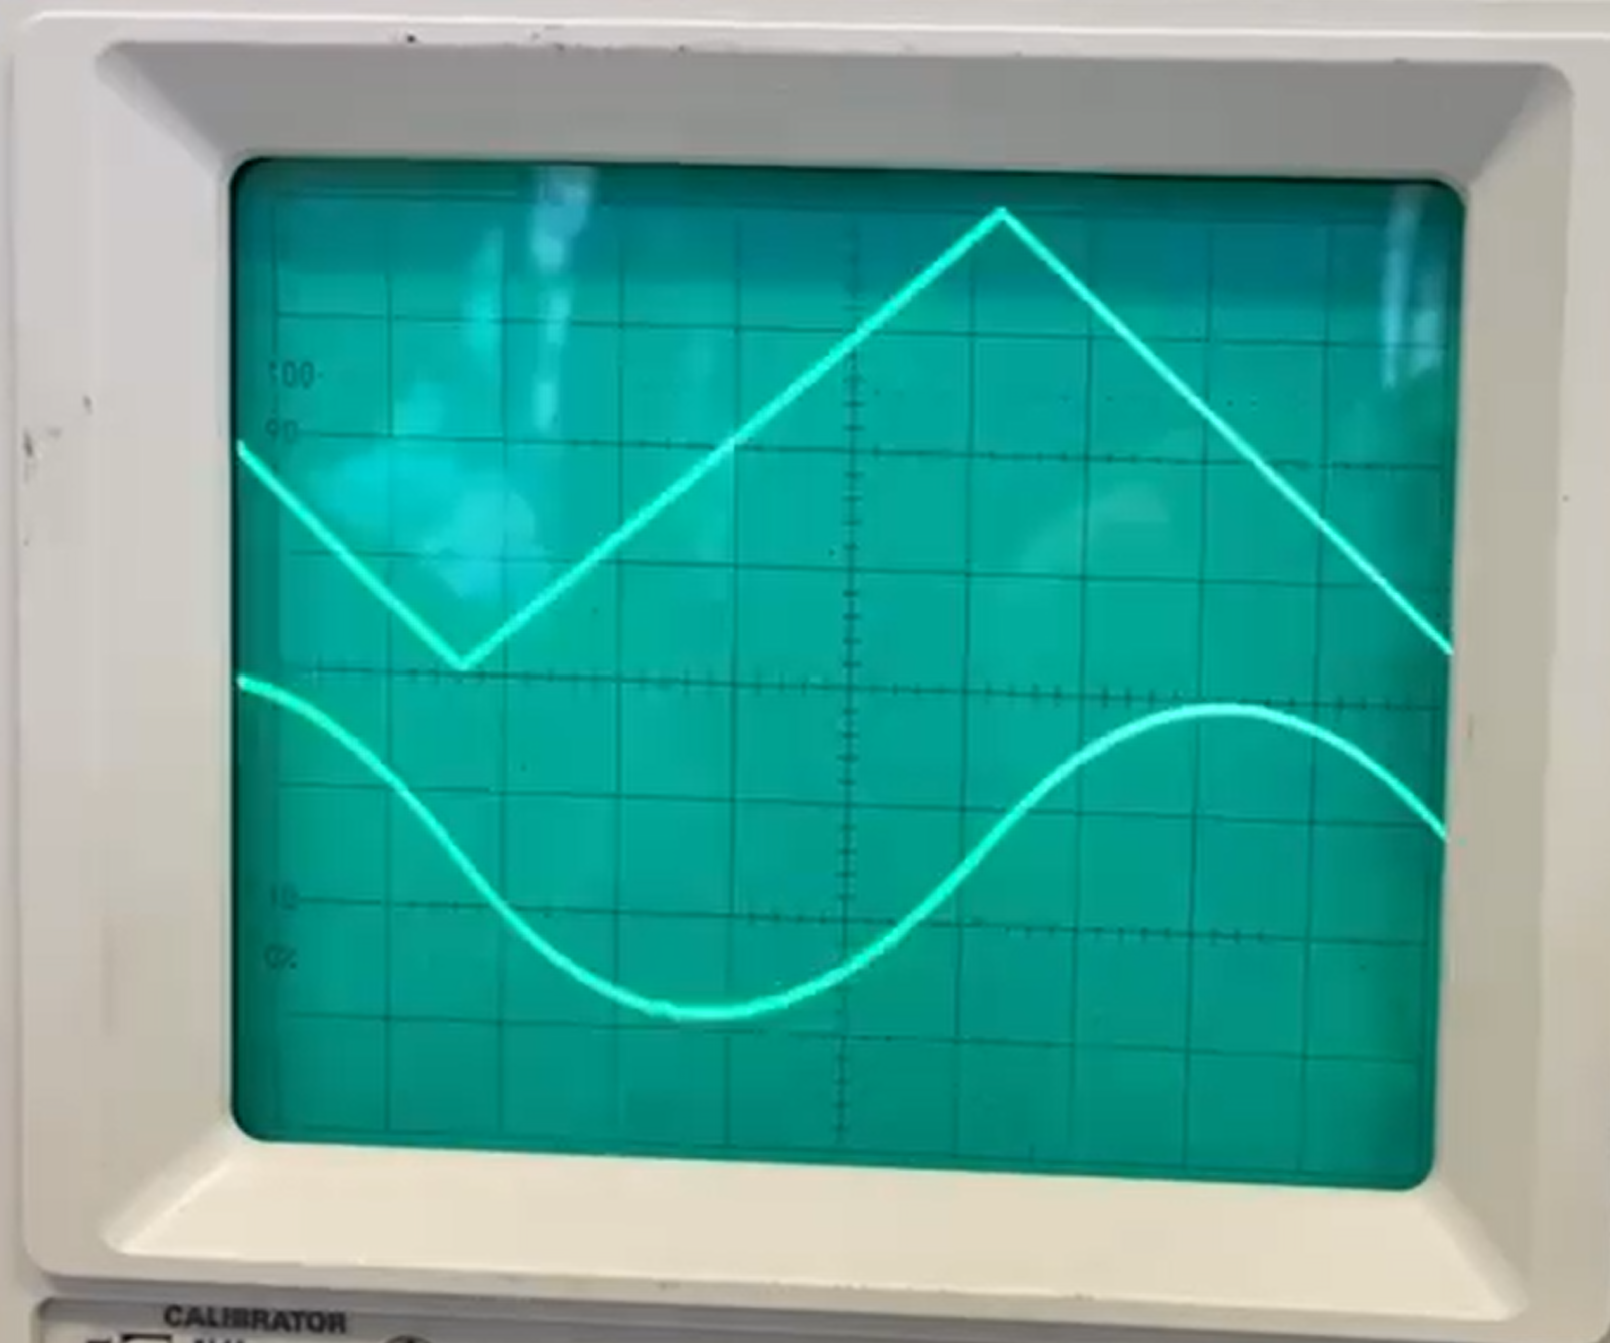
\includegraphics[height=3.5cm]{messdaten/sin_int.png}
        \caption{Dreiecksschwingung.}
    \end{subfigure}  
    \label{fig:integration}
\end{figure}   
        
         
         
         
         
         
                 
         
         
         
        